\documentclass[11pt]{article}
\usepackage[T1]{fontenc}
\usepackage[utf8]{inputenc}
\usepackage[a4paper,margin=1in]{geometry}
\usepackage{lmodern}
\usepackage{amsmath,amssymb,mathtools}
\usepackage{booktabs,longtable,array}
\usepackage{enumitem}
\usepackage{hyperref}
\usepackage{xcolor}
\usepackage{tikz}
\usetikzlibrary{arrows.meta,positioning,shapes.geometric,fit}
\hypersetup{colorlinks=true,linkcolor=blue!50!black,urlcolor=blue!50!black}

\title{Yichao v2 Brightfield-to-Fluorescence and Early Prediction Plan}
\author{OrganoidAgent}
\date{2026-06-27}

\newcommand{\B}{\mathbf{B}}
\newcommand{\F}{\mathbf{F}}
\newcommand{\M}{\mathbf{M}}
\newcommand{\Eexpr}{\mathbf{E}}
\newcommand{\R}{\mathbb{R}}
\newcommand{\argmin}{\operatorname*{arg\,min}}
\newcommand{\Dice}{\operatorname{Dice}}
\newcommand{\AUROC}{\operatorname{AUROC}}
\newcommand{\AUPRC}{\operatorname{AUPRC}}

\begin{document}
\maketitle
\tableofcontents

\section{Purpose}
The first objective is to prepare a clean Yichao v2 instance-pair database and reproduce the successful v1 brightfield-to-fluorescence result on the new data. The second objective is to extend the model from same-day prediction to early prediction:
\[
\B_{d} \mapsto \F_{d}
\qquad\text{and}\qquad
\B_{k} \mapsto \F_{d},\quad k<d .
\]
The early-prediction model should be encouraged to predict later fluorescence from earlier brightfield morphology, but it should not be over-penalized when the earliest morphology genuinely lacks enough information.

\section{Current v2 Data State}
The local v2 root is:
\begin{verbatim}
/home/lachlan/ProjectsLFS/OrganoidAgent/DATA-Yichao-v2/
\end{verbatim}

\begin{longtable}{@{}p{0.28\linewidth}p{0.23\linewidth}p{0.10\linewidth}rrrrp{0.16\linewidth}@{}}
\caption{Yichao v2 LIF inventory after copying all five files. The first two files were previously extracted and previewed; the last three were copied and metadata-inspected only.}\label{tab:v2-inventory}\\
\toprule
Folder & LIF & Day & Series & Fields & Z range & Channels & State\\
\midrule
\endfirsthead
\toprule
Folder & LIF & Day & Series & Fields & Z range & Channels & State\\
\midrule
\endhead
1\_N39Rep\_Globet\_DF\_D3 & N39Rep\_Globet\_DF\_D3.lif & D3 & 40 & 10 & 20--49 & 2 & extracted/grouped\\
2\_N39Rep\_Globet\_DF\_D4 & N39Rep\_Globet\_DF\_D4.lif & D4 & 24 & 6 & 11--38 & 2 & extracted/grouped\\
3\_N39Rep\_Globet\_DF\_D2 & N39Rep\_Globet\_DF\_D2.lif & D2 & 15 & 15 & 1 & 7 & copied/metadata\\
4\_N39Rep\_Globet\_DF\_D3\_1 & N39Rep\_Globet\_DF\_D3\_1.lif & D3 & 10 & 10 & 4--13 & 8 & copied/metadata\\
5\_N39Rep\_Globet\_DF\_D3\_2 & N39Rep\_Globet\_DF\_D3\_2.lif & D3 & 12 & 12 & 12--31 & 8 & copied/metadata\\
\bottomrule
\end{longtable}

The important structural issue is that the v2 files are not homogeneous. The already-previewed D3/D4 files contain four named acquisition series per field, such as ALEXA488, DAPI, ALEXA647, and mCherry, with two internal channels per acquisition. The newly copied D2/D3\_1/D3\_2 files contain generic \texttt{Series\#\#\#} names and seven or eight internal channels per series. Therefore, the new files require visual channel mapping before segmentation or training.

\section{Channel Mapping}
For the already-previewed named-acquisition D3/D4 files, the current practical mapping is:
\[
\text{input brightfield} = \mathrm{ALEXA488}\;c1,\qquad
\text{target fluorescence} = \mathrm{ALEXA488}\;c0.
\]
The non-ALEXA488 channels should not be treated as independent target fluorescence unless there is a biological reason. They can be used for quality control or controls.

For D2/D3\_1/D3\_2, the correct mapping is unknown. A channel contact sheet must be made before any database is built. A safe rule is:
\[
\text{no confirmed channel map} \Rightarrow \text{no segmentation database entry}.
\]

\section{Dataset Preparation Pipeline}
The preparation pipeline is intentionally separated from training.

\begin{enumerate}[leftmargin=1.5em]
  \item Inspect metadata for every LIF file.
  \item Extract all planes and group by field/series.
  \item Create channel preview grids and manually confirm brightfield and fluorescence channels.
  \item Segment the brightfield image, not the fluorescence image.
  \item Crop paired brightfield and fluorescence instances with the same segmentation mask.
  \item Store records in a v2 database with channel mapping, day, field, z policy, crop size, edge-padding flags, and split group.
\end{enumerate}

The provided preparation command is:
\begin{verbatim}
bash analysis-tools/yichao_v2/run_yichao_v2_lif_prepare.sh
\end{verbatim}
This command extracts and groups images, but it does not train and does not run segmentation.

\section{Database Design}
Each organoid crop should be represented as a single row:
\[
r = (x_B, x_F, m, d, s, z, c_B, c_F, g),
\]
where \(x_B\) is the brightfield crop, \(x_F\) is the fluorescence crop, \(m\) is the instance mask, \(d\) is day, \(s\) is source series/field, \(z\) is the z-plane or projection policy, \(c_B,c_F\) are channel identifiers, and \(g\) is the split group.

The split group is essential:
\[
g = \mathrm{donor/experiment} + \mathrm{LIF} + \mathrm{field/series} + \mathrm{replicate}.
\]
All rows with the same \(g\) must stay in the same train, validation, or test split.

\section{Same-Day Model}
The first trainable model should reproduce v1 behavior:
\[
\hat{\F}_{i,d}=f_\theta(\B_{i,d}).
\]
Use the robust v1 target style:
\begin{itemize}[leftmargin=1.5em]
  \item background-suppressed continuous fluorescence target;
  \item optional positive mask target;
  \item balanced sampling for positive signal;
  \item 256 pixel crops as the first default.
\end{itemize}

A suitable same-day loss is:
\[
\mathcal{L}_{\mathrm{same}}
=
\lambda_F \left\|\hat{\F}_{i,d}-\F^{clean}_{i,d}\right\|_1
+\lambda_M\mathcal{L}_{mask}(\hat{\M}_{i,d},\M^{clean}_{i,d})
+\lambda_E\left|\hat{E}_{i,d}-E_{i,d}\right|,
\]
where \(E_{i,d}\) is total or mean positive fluorescence.

\section{Early-to-Later Prediction}
The temporal extension is:
\[
\hat{\F}_{i,d|k}=f_\theta(\B_{i,k}, \Delta),\qquad \Delta=d-k,\quad k<d .
\]
The horizon \(\Delta\) is allowed because the requested prediction horizon is known. Future fluorescence and future brightfield are not allowed as inputs.

The full objective combines same-day and early-to-later tasks:
\[
\mathcal{L}
=
\mathcal{L}_{same}
+
\sum_{k<d} w(d-k)\mathcal{L}_{future}(i,k,d).
\]

The future loss can use the same target structure:
\[
\mathcal{L}_{future}
=
\lambda_F \left\|\hat{\F}_{i,d|k}-\F^{clean}_{i,d}\right\|_1
+\lambda_M\mathcal{L}_{mask}(\hat{\M}_{i,d|k},\M^{clean}_{i,d})
+\lambda_E\left|\hat{E}_{i,d|k}-E_{i,d}\right|.
\]

\section{Forgiving Early Horizons}
Earlier brightfield may not contain enough information. A useful objective should reward early signal when it exists but avoid forcing impossible pixel-perfect prediction.

\subsection{Fixed horizon weighting}
A simple strategy is:
\[
w(\Delta)=\exp(-\gamma \Delta).
\]
This gives near-future prediction a larger weight and very early prediction a softer weight.

\subsection{Learned uncertainty weighting}
A better strategy is:
\[
\mathcal{L}_{\Delta}
=
\frac{\mathcal{L}_{raw,\Delta}}{2\sigma_\Delta^2}
+ \log \sigma_\Delta .
\]
The model learns which horizons are intrinsically uncertain. If D2 brightfield cannot reliably predict D4 fluorescence, the objective can still learn from D3-to-D4 while not destabilizing training.

\section{No Future Leakage}
No-leakage constraints are stricter than the model architecture.

\begin{enumerate}[leftmargin=1.5em]
  \item Split by biological field/replicate before creating temporal pairs.
  \item Keep all acquisitions and days from the same split group in the same split.
  \item Use only data observed at or before day \(k\) as input for \(k\to d\).
  \item Do not normalize training inputs or tune thresholds using validation/test target distributions.
  \item Fix channel mapping before held-out evaluation.
  \item Select earliest-useful-day thresholds on validation only.
\end{enumerate}

\section{Earliest Useful Day}
For each horizon \(k\to d\), evaluate:
\begin{itemize}[leftmargin=1.5em]
  \item positive-region Dice/F1;
  \item total fluorescence Pearson or Spearman correlation;
  \item organoid-level \(\AUROC\) and \(\AUPRC\);
  \item calibration of total predicted expression.
\end{itemize}
The earliest useful day is:
\[
k^*=\min k \quad \text{such that validation metrics exceed the predefined threshold stably across replicates}.
\]

\section{Recommended Flow}
\begin{center}
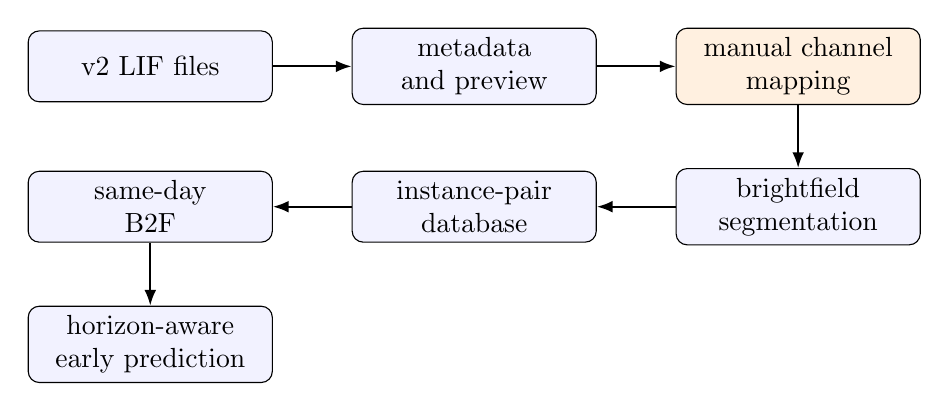
\begin{tikzpicture}[
  node distance=0.8cm and 1.0cm,
  box/.style={draw, rounded corners, align=center, minimum width=3.1cm, minimum height=0.9cm, fill=blue!5},
  warn/.style={draw, rounded corners, align=center, minimum width=3.1cm, minimum height=0.9cm, fill=orange!12},
  arrow/.style={-{Latex[length=2mm]}, thick}
]
\node[box] (lif) {v2 LIF files};
\node[box, right=of lif] (inspect) {metadata\\and preview};
\node[warn, right=of inspect] (map) {manual channel\\mapping};
\node[box, below=of map] (seg) {brightfield\\segmentation};
\node[box, left=of seg] (db) {instance-pair\\database};
\node[box, left=of db] (same) {same-day\\B2F};
\node[box, below=of same] (future) {horizon-aware\\early prediction};
\draw[arrow] (lif) -- (inspect);
\draw[arrow] (inspect) -- (map);
\draw[arrow] (map) -- (seg);
\draw[arrow] (seg) -- (db);
\draw[arrow] (db) -- (same);
\draw[arrow] (same) -- (future);
\end{tikzpicture}
\end{center}

\section{Current Decision}
Do not train immediately. The safe next step is to extract and preview the newly copied D2/D3\_1/D3\_2 files, confirm their channel mapping, and only then build the v2 segmentation/instance database.

\end{document}
